%!TEX root =../mapp-challenge-18-game-book.tex
% ^ leave for LaTeXTools build functionality

\phChapterWorksheet{Cross Products}{Cryptic Puzzle 2}

Something something Road \(\tan(87.4094^\circ)\).

\begin{center}
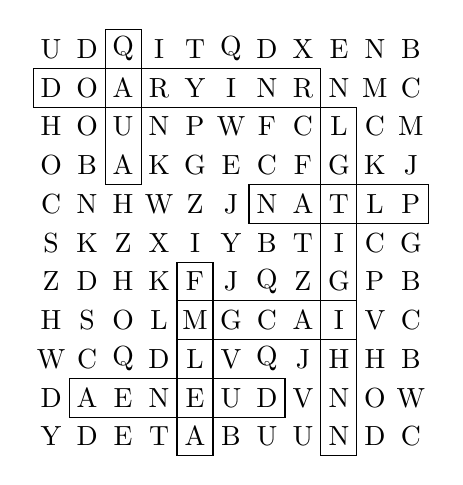
\begin{tikzpicture}[x=1.3em,y=1.4em]
  \node at (0,11) {U};\node at (1,11) {D};\node at (2,11) {Q};\node at (3,11) {I};\node at (4,11) {T};\node at (5,11) {Q};\node at (6,11) {D};\node at (7,11) {X};\node at (8,11) {E};\node at (9,11) {N};\node at (10,11) {B};
  \node at (0,10) {D};\node at (1,10) {O};\node at (2,10) {A};\node at (3,10) {R};\node at (4,10) {Y};\node at (5,10) {I};\node at (6,10) {N};\node at (7,10) {R};\node at (8,10) {N};\node at (9,10) {M};\node at (10,10) {C};
  \node at (0,9) {H};\node at (1,9) {O};\node at (2,9) {U};\node at (3,9) {N};\node at (4,9) {P};\node at (5,9) {W};\node at (6,9) {F};\node at (7,9) {C};\node at (8,9) {L};\node at (9,9) {C};\node at (10,9) {M};
  \node at (0,8) {O};\node at (1,8) {B};\node at (2,8) {A};\node at (3,8) {K};\node at (4,8) {G};\node at (5,8) {E};\node at (6,8) {C};\node at (7,8) {F};\node at (8,8) {G};\node at (9,8) {K};\node at (10,8) {J};
  \node at (0,7) {C};\node at (1,7) {N};\node at (2,7) {H};\node at (3,7) {W};\node at (4,7) {Z};\node at (5,7) {J};\node at (6,7) {N};\node at (7,7) {A};\node at (8,7) {T};\node at (9,7) {L};\node at (10,7) {P};
  \node at (0,6) {S};\node at (1,6) {K};\node at (2,6) {Z};\node at (3,6) {X};\node at (4,6) {I};\node at (5,6) {Y};\node at (6,6) {B};\node at (7,6) {T};\node at (8,6) {I};\node at (9,6) {C};\node at (10,6) {G};
  \node at (0,5) {Z};\node at (1,5) {D};\node at (2,5) {H};\node at (3,5) {K};\node at (4,5) {F};\node at (5,5) {J};\node at (6,5) {Q};\node at (7,5) {Z};\node at (8,5) {G};\node at (9,5) {P};\node at (10,5) {B};
  \node at (0,4) {H};\node at (1,4) {S};\node at (2,4) {O};\node at (3,4) {L};\node at (4,4) {M};\node at (5,4) {G};\node at (6,4) {C};\node at (7,4) {A};\node at (8,4) {I};\node at (9,4) {V};\node at (10,4) {C};
  \node at (0,3) {W};\node at (1,3) {C};\node at (2,3) {Q};\node at (3,3) {D};\node at (4,3) {L};\node at (5,3) {V};\node at (6,3) {Q};\node at (7,3) {J};\node at (8,3) {H};\node at (9,3) {H};\node at (10,3) {B};
  \node at (0,2) {D};\node at (1,2) {A};\node at (2,2) {E};\node at (3,2) {N};\node at (4,2) {E};\node at (5,2) {U};\node at (6,2) {D};\node at (7,2) {V};\node at (8,2) {N};\node at (9,2) {O};\node at (10,2) {W};
  \node at (0,1) {Y};\node at (1,1) {D};\node at (2,1) {E};\node at (3,1) {T};\node at (4,1) {A};\node at (5,1) {B};\node at (6,1) {U};\node at (7,1) {U};\node at (8,1) {N};\node at (9,1) {D};\node at (10,1) {C};

  \draw (-0.5,9.5) rectangle (7.5,10.5);
  \draw (1.5,7.5) rectangle (2.5,11.5);
  \draw (7.5,0.5) rectangle (8.5,9.5);
  \draw (5.5,6.5) rectangle (10.5,7.5);
  \draw (3.5,3.5) rectangle (8.5,4.5);
  \draw (3.5,0.5) rectangle (4.5,5.5);
  \draw (0.5,1.5) rectangle (6.5,2.5);
\end{tikzpicture}
\end{center}

(angry Dojo Master has a mixed up word search like Puzzle A in VBPuzzlehunt)


% Include below for aucTeX integration
%%% Local Variables:
%%% mode: latex
%%% TeX-master: "../mapp-challenge-18-game-book"
%%% End:
